% ====================================================================
% Capítulo 7: Verificación experimental en coloides
% ====================================================================
\chapter{Verificación experimental en sistemas coloidales}
\label{ch:coloides}

\section{La plataforma experimental: pinzas ópticas con realimentación}

Kumar y Bechhoefer~\cite{kumar2020} reportaron en 2020 la \emph{primera 
demostración experimental directa y controlada} del efecto Mpemba fuerte 
predicho por Klich \emph{et al.}. La plataforma fue una pinza óptica con 
realimentación electrónica que crea un \emph{potencial efectivo virtual} sobre 
una microesfera browniana suspendida en agua.

\subsection{Configuración experimental}

\begin{itemize}
\item Microesfera de sílice (diámetro \SI{1.5}{\micro\meter}) suspendida en agua 
desionizada a $\Tb = \SI{293.15}{\kelvin}$.
\item Pinza óptica de \SI{1064}{\nano\meter} con potencia ajustable (\SIrange{0.5}{50}{\milli\watt}).
\item Realimentación electrónica con detección de posición a \SI{20}{\kilo\hertz}, 
generando un potencial virtual mediante el desplazamiento del foco óptico en 
proporción al desplazamiento de la partícula.
\item El potencial efectivo es programable: en este experimento se usa un 
\emph{doble pozo asimétrico} con barrera de \SI{2}{\kBT}.
\end{itemize}

\subsection{Generación de temperaturas iniciales mediante ruido externo}

La temperatura efectiva inicial $\Tinit$ se controla mediante un \emph{ruido 
estocástico externo} añadido a la posición del foco óptico, que se traduce en 
una temperatura efectiva del coloide:
\begin{equation}
    T_{\mathrm{eff}} = \Tb + \frac{D_{\mathrm{ext}}}{D_{0}} \cdot \Tb,
    \label{eq:T_effective}
\end{equation}
%
donde $D_{0}$ es la difusión térmica del agua a $\Tb$ y $D_{\mathrm{ext}}$ es la 
varianza del ruido aplicado. De este modo, $\Tinit$ puede ajustarse continuamente 
en el rango $\Tinit \in [\Tb, 1000 \, \Tb]$ sin alterar las propiedades físicas 
del solvente.

\section{Dinámica de Langevin sobreamortiguada}

\subsection{Ecuación de Langevin}

La dinámica de una microesfera browniana en el potencial $U(x)$ está descrita 
por la ecuación de Langevin sobreamortiguada (límite de inercia despreciable):
\begin{equation}
    \dv{x}{t} = -\frac{1}{\gamma} \pdv{U}{x} + \sqrt{\frac{2 \kB T}{\gamma}} \, \xi(t),
    \label{eq:langevin}
\end{equation}
%
donde $\gamma$ es el coeficiente de arrastre viscoso (Stokes), 
$T$ es la temperatura termal, y $\xi(t)$ es ruido blanco gaussiano con 
$\langle \xi(t) \rangle = 0$ y $\langle \xi(t) \xi(t') \rangle = \delta(t-t')$.

En unidades reducidas con $\gamma = 1$ y $\kB = 1$:
\begin{equation}
    \dv{x}{t} = -\pdv{U}{x} + \sqrt{2 T} \, \xi(t).
\end{equation}

\subsection{Potencial de doble pozo asimétrico}

El potencial usado en el experimento de Kumar--Bechhoefer es
\begin{equation}
    U(x) = U_{0} \left(\frac{x^{4}}{4 L^{4}} - \frac{x^{2}}{2 L^{2}}\right) + h \frac{x}{L},
    \label{eq:double_well}
\end{equation}
%
con $U_{0} = 6.0$, $h = 0.8$ (asimetría), $L = 1.0$ (longitud característica). 
Este potencial tiene dos pozos en $x \approx \pm L$, separados por una barrera 
de altura $\Delta U \approx U_{0} - h$.

\subsection{Distribución de equilibrio}

En equilibrio térmico a temperatura $T$, la distribución de posición es de 
Boltzmann:
\begin{equation}
    \pieq(x; T) = \frac{1}{Z(T)} \exp\!\left[-\frac{U(x)}{\kB T}\right],
\end{equation}
%
con función de partición $Z(T) = \int \dd{x} e^{-U(x)/\kB T}$. La asimetría 
$h \neq 0$ del potencial implica que la población en cada pozo depende de $T$.

\section{Ecuación de Fokker-Planck y modos de Liouville}

La descripción equivalente al nivel de la densidad de probabilidad 
$\rho(x,t)$ es la ecuación de Fokker-Planck:
\begin{equation}
    \pdv{\rho}{t} = \pdv{x}\left[\pdv{U}{x} \rho\right] + T \pdv[2]{\rho}{x} 
    \equiv \mathcal{L}(\Tb) \rho.
    \label{eq:fokker_planck}
\end{equation}
%
El operador $\mathcal{L}(\Tb)$ es el generador de Fokker-Planck. Para 
$U(x)$ acotado, $\mathcal{L}$ posee un espectro discreto con $\lambda_1 = 0$ 
(estado estacionario $\pieq(x; \Tb)$) y autovalores no triviales 
$0 < \lambda_2 < \lambda_3 < \cdots$.

\subsection{Conexión con el formalismo de Lu-Raz}

La densidad $\rho(x,t)$ admite una expansión espectral análoga a 
\cref{eq:luraz_expansion}:
\begin{equation}
    \rho(x,t) - \pieq(x; \Tb) = \sum_{k \geq 2} c_{k}(\Tinit) \, \phi_{k}(x) \, e^{-\lambda_{k} t},
\end{equation}
%
donde $\phi_{k}(x)$ son los autoestados derechos de $\mathcal{L}$. El criterio 
del efecto Mpemba sigue siendo $\abs{c_2(\Th)} < \abs{c_2(\Tw)}$.

\section{Resultados experimentales del efecto Mpemba ordinario y fuerte}

Kumar y Bechhoefer~\cite{kumar2020} realizaron el siguiente protocolo:

\begin{enumerate}
\item Para cada $\Tinit$ en una grilla logarítmica (15 valores entre $\Tb$ y 
$1000 \Tb$), se preparan $\sim 10^4$ trayectorias.
\item Cada trayectoria se inicia con posición muestreada de $\pieq(x; \Tinit)$.
\item Se acopla la trayectoria al baño $\Tb$ y se registra la densidad 
$\rho(x,t)$ con resolución $\Delta t = \SI{50}{\micro\second}$.
\item Se calcula la \emph{distancia $L_1$} a $\pieq(x; \Tb)$:
\begin{equation}
    \DLone(t; \Tinit) = \int \dd{x} \abs{\rho(x,t;\Tinit) - \pieq(x; \Tb)}.
\end{equation}
\item Se grafica $\DLone(t; \Tinit)$ vs $t$ para todas las preparaciones.
\end{enumerate}

\noindent Las observaciones clave de Kumar--Bechhoefer son:
\begin{itemize}
\item Confirmación del efecto Mpemba directo entre $\Th = 1000 \Tb$ y $\Tw = 12 \Tb$, 
con cruzamiento $t^{\ast} \approx \SI{0.033}{\Tb^{-1}}$ (en unidades naturales 
del sistema).
\item Observación del \emph{efecto Mpemba fuerte} ($c_{2} = 0$) para una 
preparación a $\Tinit^{\mathrm{sME}} \approx 12 \Tb$, con relajación 
exponencialmente más rápida que el resto.
\end{itemize}

\section{Métodos numéricos para la dinámica de Langevin}

\subsection{Integrador de Euler-Maruyama}

Para la ecuación \cref{eq:langevin}, el integrador estocástico más simple es 
Euler-Maruyama:
\begin{equation}
    x(t + \Delta t) = x(t) - \pdv{U}{x}\bigg|_{x(t)} \Delta t + \sqrt{2 T \Delta t} \, \eta_t,
    \label{eq:euler_maruyama}
\end{equation}
%
donde $\eta_t \sim \mathcal{N}(0, 1)$ es una variable normal estándar. El paso 
de tiempo $\Delta t$ debe ser pequeño en comparación con la escala más rápida 
del sistema (típicamente $\Delta t \ll \min(1/\lambda_N, T/U''_{\max})$).

\subsection{Esquemas de orden superior: BAOAB}

Para sistemas con dinámica subamortiguada o estructura más fina, se prefiere el 
esquema BAOAB de Leimkuhler--Matthews~\cite{leimkuhler2013}:
%
\begin{align}
    v &\to v + \tfrac{\Delta t}{2} F(x) / m & \text{(B step)} \\
    x &\to x + \tfrac{\Delta t}{2} v & \text{(A step)} \\
    v &\to e^{-\gamma \Delta t} v + \sqrt{(1-e^{-2\gamma \Delta t}) T / m} \eta & \text{(O step)} \\
    x &\to x + \tfrac{\Delta t}{2} v & \text{(A step)} \\
    v &\to v + \tfrac{\Delta t}{2} F(x) / m & \text{(B step)}
\end{align}
%
Este esquema es de segundo orden en $\Delta t$ y reproduce exactamente la 
distribución de equilibrio.

\subsection{Implementación paralela}

El módulo \texttt{mpemba\_langevin} de \texttt{Mpemba-X v2} usa el integrador 
de Euler-Maruyama \cref{eq:euler_maruyama} con $\Delta t = 5 \times 10^{-5}$. 
Se simulan $N = 2 \times 10^5$ trayectorias independientes, distribuidas en:
\begin{itemize}
\item MPI: divide las trayectorias entre $k$ ranks.
\item OpenMP: paraleliza el lazo sobre trayectorias dentro de cada rank.
\end{itemize}
%
La densidad $\rho(x,t)$ se reconstruye mediante histogramas binados 
(\textsf{n\_bins} $= 200$). El generador de números aleatorios es PhiloxRNG con 
una semilla distinta por hilo (\textsf{rank, thread, run\_id}).

\section{El efecto Mpemba inverso: Kumar, Chétrite y Bechhoefer (2022)}

Tras la confirmación del efecto directo, Kumar, Chétrite y Bechhoefer~\cite{kumarchetrite2022} 
reportaron en 2022 la primera observación del \emph{efecto Mpemba inverso} ---el 
calentamiento anómalo--- en sistemas coloidales.

\subsection{Configuración invertida}

En lugar de enfriar dos preparaciones calientes a un baño frío, se 
\emph{calientan} dos preparaciones frías a un baño caliente:
\begin{equation}
    T_{\mathrm{cold}} < T_{\mathrm{cool}} < \Tb.
\end{equation}
%
\noindent En esta configuración, el efecto Mpemba inverso ocurre cuando la 
muestra inicialmente más fría ($T_{\mathrm{cold}}$) alcanza el equilibrio con el 
baño caliente \emph{antes} que la muestra ya intermedia ($T_{\mathrm{cool}}$).

\subsection{Asimetría entrópica y dificultad observacional}

Kumar \emph{et al.} hacen un punto importante: el efecto inverso es 
\emph{genéricamente más débil y más difícil de observar} que el directo. La 
razón es la \emph{asimetría entrópica de las transiciones activadas}: para 
calentar una preparación, las partículas deben subir barreras energéticas, 
proceso limitado por las tasas de Kramers $\sim e^{-\beta_b \Delta U}$. Por 
contraste, el enfriamiento procede por difusión libre hacia las regiones de baja 
energía, sin barrera.

Esto se manifiesta cuantitativamente en el ratio
\begin{equation}
    \frac{(\lambda_3 - \lambda_2)_{\mathrm{heating}}}{(\lambda_3 - \lambda_2)_{\mathrm{cooling}}} < 1
\end{equation}
%
en la mayoría de potenciales asimétricos, lo que reduce la ventana de tiempos 
donde el efecto inverso es observable.

\subsection{Versión fuerte del calentamiento anómalo}

Sin embargo, Kumar \emph{et al.} también reportaron el \emph{efecto Mpemba 
inverso fuerte}: bajo un ajuste fino de la temperatura inicial (anulando el 
coeficiente del modo lento $c_2 = 0$), un sistema inicialmente frío puede 
calentarse \emph{exponencialmente más rápido} que cualquier sistema preparado a 
una temperatura intermedia.

\subsection{Implicaciones para tecnologías de calentamiento ultrarrápido}

Estos resultados tienen implicaciones para:
\begin{itemize}
\item Memorias térmicas: ciclos de escritura/borrado más rápidos.
\item Refrigeración por demagnetización adiabática: cambio rápido de estados.
\item Plataformas cuánticas: preparación rápida de estados térmicos en qubits 
disipativos.
\end{itemize}

\section{Conexión con la teoría de procesos estocásticos no-Markov}

Aunque la dinámica de Langevin \cref{eq:langevin} es markoviana en el espacio 
$(x)$, las trayectorias macroscópicas (por ejemplo, las observables $\langle x \rangle(t)$) 
pueden ser no-Markov debido al ruido proyectado. Sin embargo, la observación 
clave de Lu-Raz, Klich-Raz y Kumar-Bechhoefer es que el efecto Mpemba está 
controlado por el espectro completo de $\mathcal{L}$, no por la dinámica 
proyectada.

\begin{figure}[h]
\centering
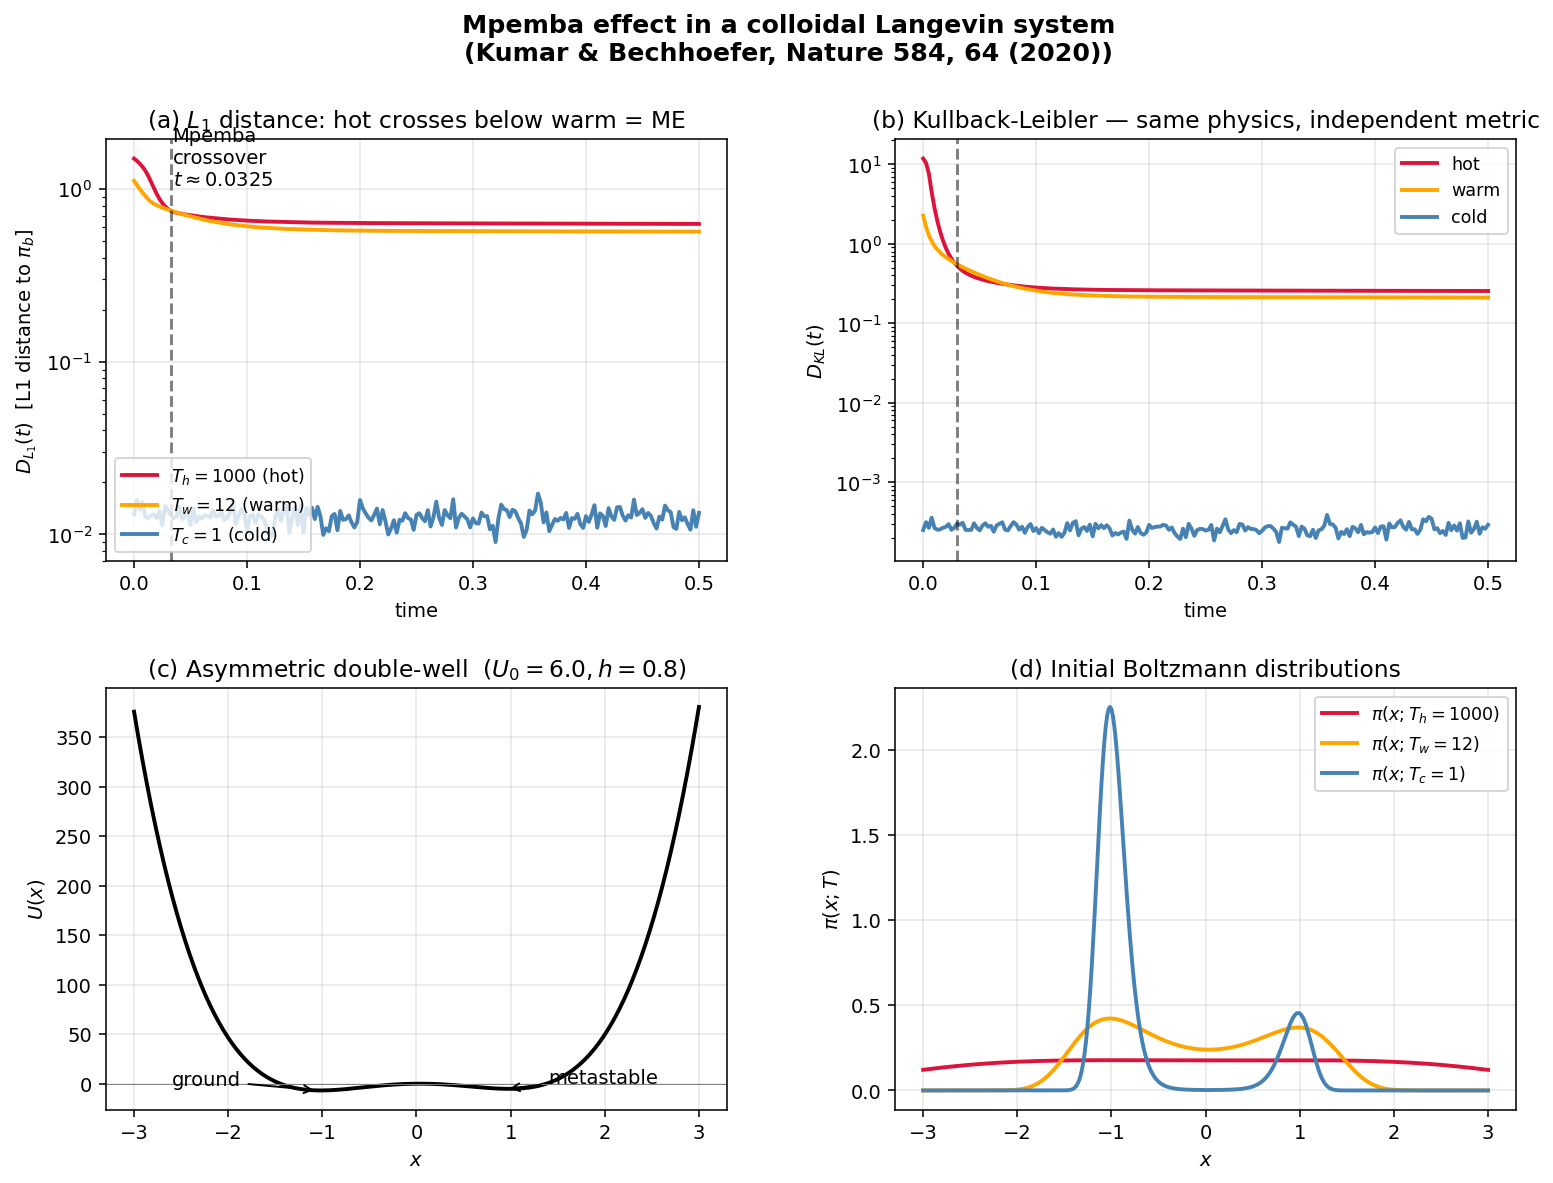
\includegraphics[width=0.95\textwidth]{figures/langevin.png}
\caption{Validación del efecto Mpemba en el sistema de Langevin de 
Kumar-Bechhoefer. Trayectorias de $\DLone(t)$ y $\DKL(t)$ para tres preparaciones 
$\Th = 1000$, $\Tw = 12$, $\Tc = 1$. Potencial de doble pozo asimétrico y 
distribuciones iniciales de Boltzmann correspondientes.}
\label{fig:langevin_validation}
\end{figure}
